\documentclass[11pt,oneside]{article}
\usepackage[T1]{fontenc}
\usepackage[utf8]{inputenc}
%\DeclareUnicodeCharacter{00A0}{ }
\usepackage[adobe-utopia]{mathdesign}

\usepackage{amsmath}
\usepackage[francais]{babel}
\usepackage[dvips]{graphicx}
%\usepackage{here}
\usepackage{framed}
\usepackage[normalem]{ulem}
\usepackage{fancyhdr}
\usepackage{titlesec}
\usepackage{vmargin}

\usepackage{amsmath}
\usepackage{ifthen}
\usepackage{multirow}
\usepackage{multicol} % Portions de texte en colonnes

%\usepackage{xltxtra} % Logo XeLaTeX
%\usepackage{pst-solides3d}
\usepackage{color}
%\usepackage{colortbl}
\usepackage{titletoc} % Pour la mise en forme de la table des matières

%\usepackage[crop=off]{auto-pst-pdf}
%\usepackage{bclogo}


%\usepackage{longtable}
%\usepackage{flafter}%floatants après la référence
%\usepackage{pst-solides3d}
%\usepackage{pstricks}
%\usepackage{minitoc}
%\setcounter{minitocdepth}{4}
%\usepackage{draftcopy}% "Brouillon"
%\usepackage{floatflt}
%\usepackage{psfrag}
%\usepackage{listings} % Permet d'insérer du code de programmation
%\usepackage{lmodern}
%\usepackage[adobe-utopia,uppercase=upright,greeklowercase=upright]{mathdesign}
%\usepackage{minionpro}
%\usepackage{pifont}
%\usepackage{amssymb}
%\usepackage[francais]{varioref}

\setmarginsrb{1.5cm}{1cm}{1cm}{1.5cm}{1cm}{1cm}{1cm}{1cm}

\definecolor{gris25}{gray}{0.75}
\definecolor{bleu}{RGB}{18,33,98}
\definecolor{bleuf}{RGB}{42,94,171}
\definecolor{bleuc}{RGB}{231,239,247}
\definecolor{rougef}{RGB}{185,18,27}
\definecolor{rougec}{RGB}{255,230,231}
\definecolor{vertf}{RGB}{103,126,82}
\definecolor{vertc}{RGB}{220,255,191}
\definecolor{violetf}{RGB}{112,48,160}
\definecolor{violetc}{RGB}{230,224,236}
\definecolor{jaunec}{RGB}{220,255,191}
\usepackage[raccourcis]{FAST}
\usepackage[%
    pdftitle={Systèmes à événements discrets},
    pdfauthor={Xavier Pessoles},
    colorlinks=true,
    linkcolor=blue,
    citecolor=magenta]{hyperref}
\usepackage{schemabloc}



% \makeatletter \let\ps@plain\ps@empty \makeatother
%% DEBUT DU DOCUMENT
%% =================
\sloppy
\hyphenpenalty 10000

\newcommand{\Pointilles}[1][3]{%
\multido{}{#1}{\makebox[\linewidth]{\dotfill}\\[\parskip]
}}


\colorlet{shadecolor}{orange!15}

\newtheorem{theorem}{Theorem}


\begin{document}


\newboolean{prof}
\setboolean{prof}{true}
%------------- En tetes et Pieds de Pages ------------
\pagestyle{fancy}
\renewcommand{\headrulewidth}{0pt}

\fancyhead{}
\fancyhead[L]{%
\noindent\noindent\begin{minipage}[c]{2.6cm}
%Lycée Rouvière PTSI

\includegraphics[width=2cm]{png/logo_ptsi.png}%
\end{minipage}
}

\fancyhead[C]{\rule{12cm}{.5pt}}

\fancyhead[R]{%
\noindent\begin{minipage}[c]{3cm}
\begin{flushright}
\footnotesize{\textit{\textsf{Sciences Industrielles\\ pour l'Ingénieur}}}%
\end{flushright}
\end{minipage}
}

\renewcommand{\footrulewidth}{0.2pt}

\fancyfoot[C]{\footnotesize{\bfseries \thepage}}
\fancyfoot[L]{\footnotesize{2012 -- 2013} \\ X. \textsc{Pessoles}}
\ifthenelse{\boolean{prof}}{%
\fancyfoot[R]{\footnotesize{Cours -- CI 8 : SED -- P}}
}{%
\fancyfoot[R]{\footnotesize{Cours -- CI 8 : SED}}
}



\begin{center}
 \huge\textsc{CI 8 -- SED -- Systèmes à événements discrets}

 \large\textsc{Commande et comportement des systèmes combinatoires et séquentiels}
\end{center}

\begin{center}
 \LARGE\textsc{Chapitre 1 -- Étude des systèmes combinatoires}
\end{center}


\vspace{.5cm}
\begin{flushright}
\textit{D'après ressources de David Violeau et Florestan Mathurin}
\end{flushright}
%\begin{center}
%\begin{tabular}{cccc}
%\includegraphics[height=2.5cm]{png/acier} &
%\includegraphics[height=2.5cm]{png/bois} &
%\includegraphics[height=2.5cm]{png/composite} &
%\includegraphics[height=2.5cm]{png/verre}\\
%\textit{Acier \cite{acier}} & 
%\textit{Bois} & 
%\textit{Fibre de carbone \cite{composite}} & 
%\textit{Verre \cite{verre}} \\
%\end{tabular}
%\end{center}



Un des objectifs de l'automaticien est de concevoir la partie commande qui traite les informations et élabore les ordres. Ce cours étudie le cas où les informations et les ordres élaborés sont des variables binaires.
\begin{prob}
\textsc{Problématique :}

%En phase d'avant conception d'un produit, quels sont les critères qui vont permettre de choisir les matériaux à utiliser ?
\end{prob}

\begin{savoir}
\textsc{Savoirs :}
\begin{itemize}
\item Exprimer le fonctionnement d'un système combinatoire sous forme d'équations logiques
\item Optimiser la représentation logique du système
\item Décrire, au moyen d'une représentation adaptée, le comportement du système
\end{itemize}
\end{savoir}

%\newpage 

\setlength{\parskip}{0ex plus 0.2ex minus 0ex}
 \renewcommand{\contentsname}{}
 \renewcommand{\baselinestretch}{1}

\tableofcontents

 \renewcommand{\baselinestretch}{1.2}
\setlength{\parskip}{2ex plus 0.5ex minus 0.2ex}

% \vspace{1cm}
\textit{Ce document évolue. Merci de signaler toutes erreurs ou coquilles.}




\section{Numération et codage}
Le système de numérotation le plus utilisé aujourd'hui et le système décimal. Les systèmes automatiques utilisent plus naturellement le système binaire. La connaissance du système binaire et des changements de base binaire vers décimal et décimal vers binaire est donc essentielle à l'étude et à la réalisation des parties commandes.

\subsection{Système de numération}
\subsubsection{Bases}

\begin{minipage}[c]{.45\linewidth}
Un nombre est représenté par la juxtaposition de symboles appelés digits pris parmi les éléments de la base $\mathcal{B}$ considérée.

Les vases les plus couramment utilisées sont :
\begin{itemize}
\item la base 10 (ou décimale) contenant 10 symboles : 0, 1, 2, 3, 4, 5, 6, 7, 8, 9;
\item la base 2 (ou binaire) contenant 2 symboles : 0, 1;
\item la base 16 (ou hexadécimale) comprenant 16 symboles : 0, 1, 2, 3, 4, 5, 6, 7, 8, 9, A, B, C, D, E, F. 
\end{itemize}
\end{minipage}\hfill
\begin{minipage}[c]{.45\linewidth}
\begin{center}
\begin{tabular}{|c|c|c|}
\hline
Base décimale & 
Base binaire & 
Base hexadécimale \\
$\mathcal{B}_{10}$ & 
$\mathcal{B}_{2}$ & 
$\mathcal{B}_{16}$ \\
\hline \hline
0 & \texttt{0000} & \texttt{0} \\ \hline
1 & \texttt{0001} & \texttt{1} \\ \hline
2 & \texttt{0010} & \texttt{2} \\ \hline
3 & \texttt{0011} & \texttt{3} \\ \hline
4 & \texttt{0100} & \texttt{4} \\ \hline
5 & \texttt{0101} & \texttt{5} \\ \hline
6 & \texttt{0110} & \texttt{6} \\ \hline
7 & \texttt{0111} & \texttt{7} \\ \hline
8 & \texttt{1000} & \texttt{8} \\ \hline
9 & \texttt{1001} & \texttt{9} \\ \hline
10 & \texttt{1010} & \texttt{A} \\ \hline
11 & \texttt{1011} & \texttt{B} \\ \hline
12 & \texttt{1100} & \texttt{C} \\ \hline
13 & \texttt{1101} & \texttt{D} \\ \hline
14 & \texttt{1110} & \texttt{E} \\ \hline
15 & \texttt{1111} & \texttt{F} \\ \hline
\end{tabular}
\end{center}
\end{minipage}


\subsubsection{Changement de base : transcodage}
L'objectif est de mettre en place la correspondance entre l'expression d'un nombre dans une base et son expression dans une autre base. 

\begin{methode}
\textbf{Passage d'une base $X$ vers la base décimale}

Notons $a$, $b$, $c$ et $d$ 4 digits et $X$ une base quelconque. Pour obtenir $(abcd)_X$ dans la base décimale, il faut d'abord connaître la correspondance entre les digits des bases $X$ et 10. La méthode est alors la suivante : 
$$
(abcd)_X  = a_{10}\cdot X^3 + b_{10}\cdot X^2 + c_{10}\cdot X^1 + d_{10}\cdot X^0
$$

On parle de système de numération pondéré. On appelle poids le rang de chaque digit. ($a$ est le digit de poids le plus fort).
\end{methode}

\begin{exemple}
Passer les nombres suivants en base décimale : $(1011)_2$ et $(A3B)_{16}$.
\end{exemple}

\begin{methode}
\textbf{Passage d'une base décimale vers la base $X$}

On utilise la méthode des divisions successives. Soit un nombre $N$ défini sur une base $X$. Son écriture en base 10 est la suivante : 
$$
(N)_X = n_{p} \cdot x^{p} + n_{p-1} \cdot x^{p-1} + ... +  n_{1} \cdot x^{1} +  n_{0} \cdot x^{0}
$$

Effectuer le changement de base revient à déterminer les coefficients $n_i$.

\end{methode}


En mettant $x$ en facteur il vient : 

$$
(N)_X =x\cdot\left( n_{p} \cdot x^{p-1} + n_{p-1} \cdot x^{p-2} + ... +  n_{1} \cdot x^{0}\right) +  n_{0} 
$$

Cette expression est de la forme $(N)_X = x(\text{quotient}) + \text{reste}$. Le reste permet donc de déterminer $n_0$. 

\begin{minipage}[c]{.45\linewidth}

En reprenant le quotient précédent et en factorisant par $x$ on trouve un nouveau reste $n_1$ et ainsi de suite jusqu'à $n_p$. 

Ainsi pour écrire un nombre décimal en binaire, il faut faire des divisions successives par 2. Par exemple pour écrire 19 en binaire, on réalise les divisions ci-contre. 

Le sens de lecture, et donc d'écriture se fait selon la flèche. On a donc $(19)_{10}=1\;0011$.

\end{minipage} \hfill
\begin{minipage}[c]{.45\linewidth}
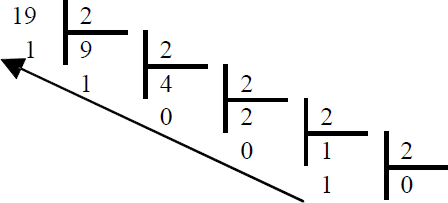
\includegraphics[width=.8\textwidth]{png/fig_01}
\end{minipage} 

\begin{exemple}
Écrire 25 en binaire et en hexadécimal. 
\end{exemple}
%\newpage

\subsection{Codage de l'information} 

Les ordinateurs travaillant en binaire, tout traitement informatique ou automatique nécessite de coder l'information en binaire à l'aide de deux états 1 ou 0. Un bit (contraction de binary digit) est un chiffre binaire (1 ou 0). un octet (byte en anglais) correspond à 8 bits. Un ko (kilo octet) correspond à $2^{10}$ chiffres soit 1024 octets.

L'écriture des nombres dans cette base donnant une multitude de chiffres, les informaticiens lui préfèrent le système hexadécimal qui permet de contracter les informations en paquets de 4 bits. 

Il est également intéressant de regrouper un ensemble de valeurs binaires suivant une autre organisation qu'un système de nombres. Cette organisation sont appelées codes. Il en existe un très grand nombre et chacun peut en créer selon un besoin spécifique.

Les qualités requises pour un code sont principalement :
\begin{itemize}
\item la taille du codage (nombre de bits nécessaires);
\item la fiabilité de lecture;
\item la simplification de manipulation.
\end{itemize}

\begin{exemple}
\begin{minipage}[c]{.7\linewidth}
Sur une carte vitale, les données sont codées selon la norme ASCII (American Standard Code For Information Interchange) qui nécessite 8 bits et permet de coder 256 caractères. Les chiffre de 0 à 9 en ASCII binaire sont obtenus en ajoutant 0011 devant le code binaire du chiffre sur 4 bits. Les lettres de A à Z sont codées en ajoutant 010 devant le code binaire des 26 lettres (A=01000001, \textit{etc}).
\end{minipage}\hfill
\begin{minipage}[c]{.25\linewidth}
\begin{center}
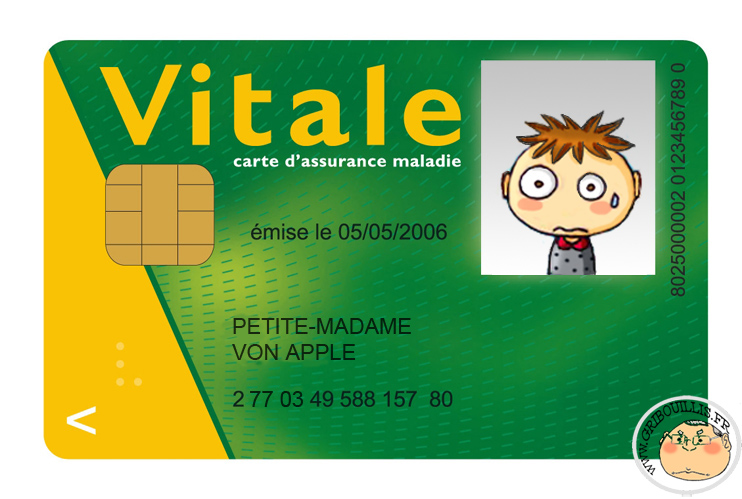
\includegraphics[width=.8\textwidth]{png/fig_02}
\end{center}
\end{minipage}
\end{exemple}

\begin{exemple}
Écrire la séquence suivante en ASCII binaire : 19 ans. Combien d'octets sont nécessaires pour coder cette séquence ?

\end{exemple}

On étudie dans la suite les principaux codes à connaître. On distingue les codes pondérés pour lesquels chaque chiffre possède un poids, des codes non pondérés qui nécessitent une table de correspondance pour décoder un nombre. 

\subsubsection{Code binaire naturel}
Ce code pondéré correspond à donner un nombre selon sa valeur en système de numérotation binaire. 

C'est le seul code qui permet de réaliser des opérations. 

Inconvénient : il introduit des erreurs lors d'un changement de code. Pour passer de $(01)_2$ à $(10)_2$, donc de 1 à2, il faut modifier chaque digit et afficher (même brièvement) $(11)_2$ (soit 3) ou $(00)_2$ (soit 0). Cela peut provoquer des perturbations ou des erreurs. 

\begin{center}
\begin{tabular}{|c|c|c|c||c|}
\hline
\multicolumn{4}{|c|}{Entrée} & Sortie \\ \hline \hline
0 & 0 & 0 & 0 & 0 \\ \hline 
0 & 0 & 0 & 1 & 1 \\ \hline
0 & 0 & 1 & 0 & 2 \\ \hline
0 & 0 & 1 & 1 & 3 \\ \hline
0 & 1 & 0 & 0 & 4 \\ \hline
0 & 1 & 0 & 1 & 5 \\ \hline
0 & 1 & 1 & 0 & 6 \\ \hline
0 & 1 & 1 & 1 & 7 \\ \hline
1 & 0 & 0 & 0 & 8 \\ \hline
1 & 0 & 0 & 1 & 9 \\ \hline
\end{tabular}

\textit{Table de vérité du code binaire naturel}
\end{center} 


\subsubsection{Code décimal codé binaire (DCB)}
C'est un code pondéré base sur le code binaire naturel mais qui est adapté à la représentation des nombres en base 10. En effet le code binaire pur n'associe pas des bits spécifiques aux unités, dizaines, centaines, ... La propriété du code DCB est d'associer 4 bits différents à chaque puissance de 10. Ainsi, 
$$
(1664)_{10} \quad \Longrightarrow \quad  (0001.0110.0110.0100)_{DCB}
$$

Ce code est utilisé pour les afficheurs 7 segments. Chaque afficheur reçoit le chiffre codé en binaire sur 4 bits. 

\begin{minipage}[c]{.6\linewidth}
Inconvénient : Cette représentation adaptée à la représentation binaire des nombres décimaux utilise un nombre de bits supérieur à celui du binaire naturel, et donc une place plus important en mémoire de l'ordinateur. 
\end{minipage} \hfill
\begin{minipage}[c]{.25\linewidth}
\begin{center}
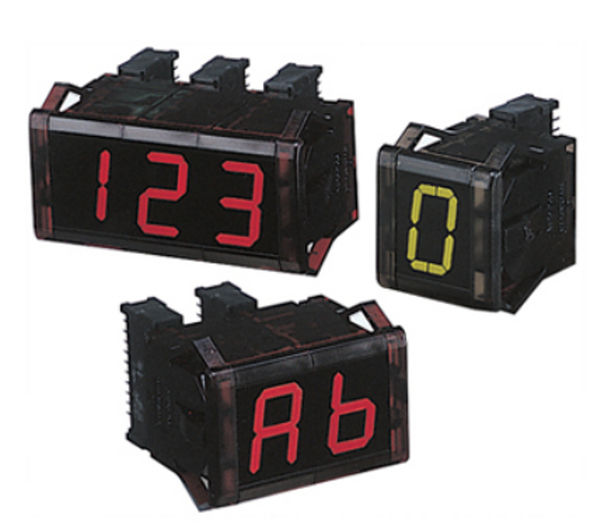
\includegraphics[width=.8\textwidth]{png/fig_03}
\end{center}
\end{minipage}

\begin{rem}
On peut réaliser la même typologie pour le code hexadécimal. Notons ce codage HCB. Ainsi,
$$
(0C3F)_{16} \quad \Longrightarrow \quad (0000.1100.0011.1111)_{HCB}
$$
\end{rem}

\subsubsection{Code  binaire réfléchi ou code Gray}
Ce code non pondéré est un arrangement du système binaire. Le passage d'un nombre à l'autre se fait en changeant l'état d'un seul bit. Il est très utilisé pour décrire des automatismes (un changement d'état d'un composant correspond à un bit qui change), en particulier dans les codeurs de position absolue. 

Avantage : il apporte une garantie d'interprétation avec une erreur maximale d'incrémentation. 

\begin{center}
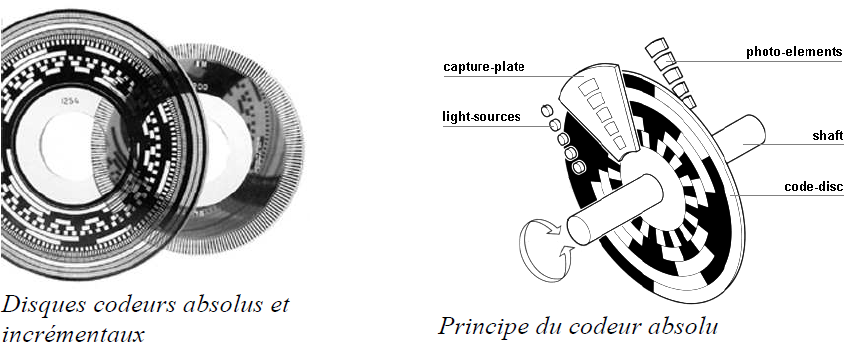
\includegraphics[width=.7\textwidth]{png/fig_04}
\end{center}

Pour obtenir le code Gray, il faut faire toutes les $2^1$, $2^2$, $2^3$ ... lignes, une symétrie en commençant par le bit de droite et changer la valeur du bit de gauche. 

\begin{center}
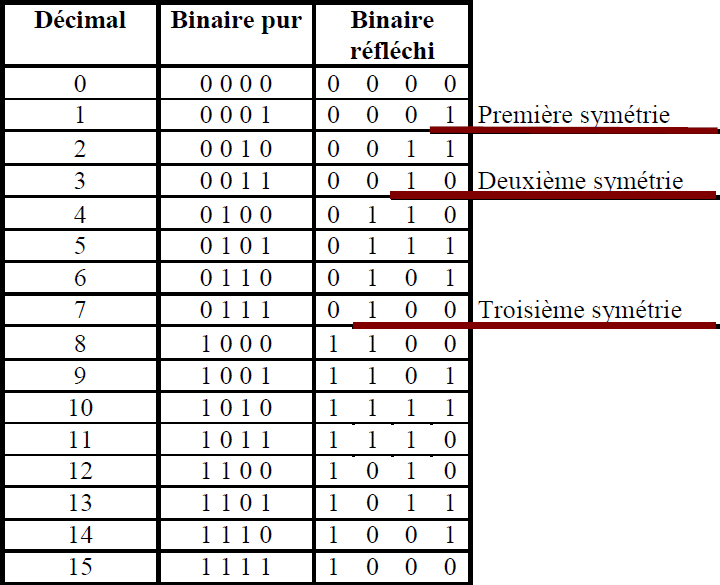
\includegraphics[width=.7\textwidth]{png/fig_05}
\end{center}

%\begin{exemple}
%Écrire en code Gray le nombre 56.
%\end{exemple}


\section{Systèmes combinatoires}

\begin{exemple}
Support : éclairage d'un escalier

On souhaite éclairer un escalier par 4 lampes qui s'allument automatiquement lorsque l'on monte ou descend l'escalier. Pour l'esthétisme, on désire que les lampes s'allument puis s'éteignent successivement lorsqu'une présence est détectée. On utilise 3 détecteurs de présence notés $a$, $b$, et $c$. L'objectif est de déterminer les équations logiques liant l'état des lampes à l'état des détecteurs de présence. Chaque capteur détecte une présence. Chaque capteur détecte une présence dans la zone indiquée. Il faut toujours 2 lampes d'allumées sauf aux marches extrêmes. 
\end{exemple}


\begin{center}
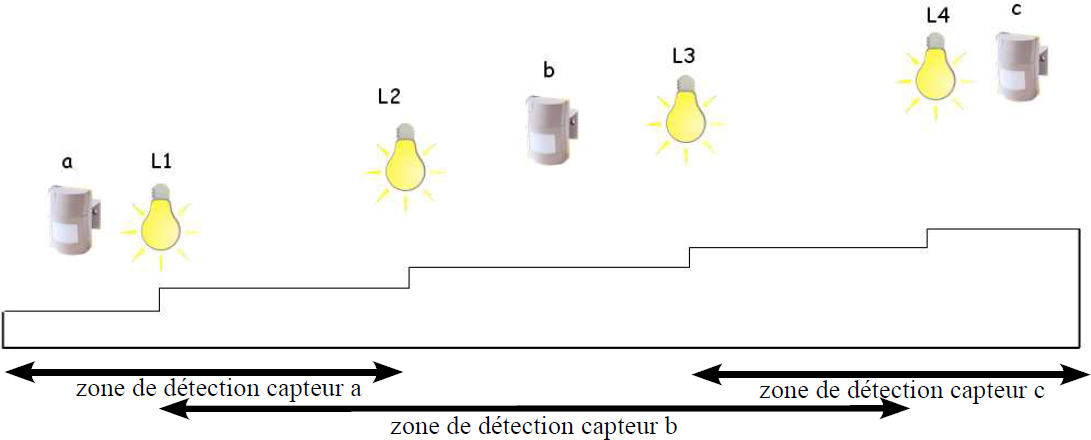
\includegraphics[width=.9\textwidth]{png/fig_06}
\end{center}


\subsection{Définitions}
\subsubsection{Variables binaires}
De nombreux composants utilisés en automatisme ne peuvent normalement prendre que deux états différents : lampe allumée ou éteinte, bouton-poussoir actionné ou relâché, moteur tournant ou à l'arrêt, vérin pneumatique sorti ou rentré. 


A chacun de ces composants, on peut associer une variable binaire (ou logique, Tout Ou Rien) qui ne peut prendre que deux valeurs notées 0 ou 1 (vrai ou faux, oui ou non). 

\begin{defi}
Une variable $a$ est binaire si et seulement si elle peut prendre, à chaque instant, qu'une seule valeur parmi un ensemble de 2 valeurs possibles. 
\end{defi}

\begin{exemple}
\textit{Lister les variables binaires pour l'éclairage de l'escalier}
\end{exemple}

\begin{rem}
Le comportement tout ou rien (TOR) ne correspond qu'au comportement normalement prévu en régime stabilisé et en l'absence de tout dysfonctionnement. 

L'association d'une variable binaire à un composant ne peut pas rendre compte des états transitoires apparaissent entre deux états stables. C'est donc une simplification du comportement réel.
\end{rem}


\begin{center}
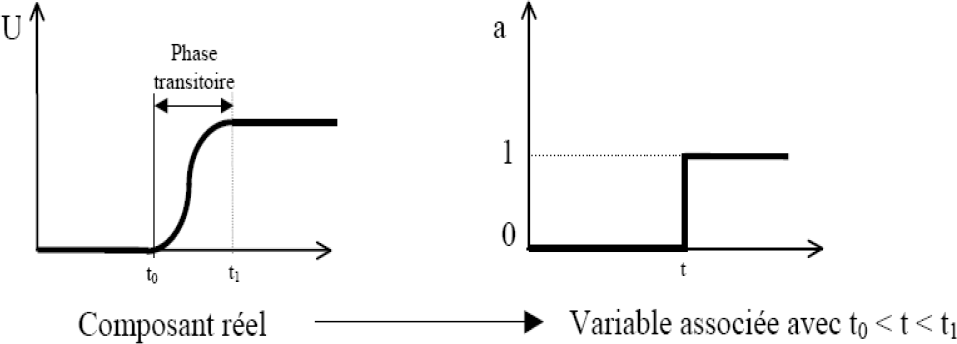
\includegraphics[width=.8\textwidth]{png/fig_07}
\end{center}

\subsubsection{Système binaire}

\begin{defi}
Un système est dit binaire ou logique si les variables d'entrée et de sortie sont binaires. 
\end{defi}

\subsubsection{Systèmes combinatoire et séquentiel}
\begin{defi}
Un système logique combinatoire est un système binaire pour lequel à un état des variables d'entrée $E_i$ correspond un unique état des variables de sortie $S_j$. (La réciproque n'est pas vraie.)
\end{defi}

\begin{center}
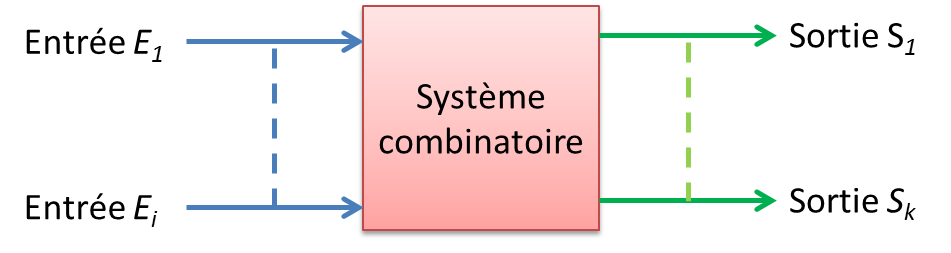
\includegraphics[width=.6\textwidth]{png/fig_08}
\end{center}

\begin{defi}
Un système logique est dit séquentiel si les sorties $S_j$ ne dépendent pas uniquement des $E_i$.
\end{defi}

\begin{exemple}
\begin{center}
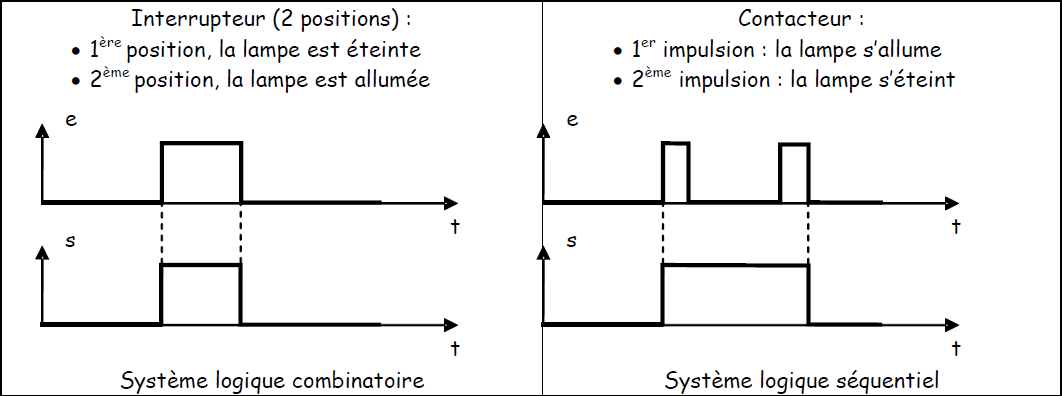
\includegraphics[width=.9\textwidth]{png/fig_09}
\end{center}

\end{exemple}


\subsection{Algèbre de Boole}

La fonction logique qui caractérise le système est indépendante du temps. Pour traiter de tels systèmes, on utilise l'algèbre de Boole. 

\subsubsection{Définition}
C'est un algèbre de propositions logiques mise au point par un mathématicien anglais, Georges Boole (1815 -- 1864).

\begin{defi}
Un ensemble $E$ a une structure d'algèbre Boole si on a défini dans cet ensemble :
\begin{itemize}
\item une relation d'équivalence notée $=$;
\item deux lois de composition interne $+$ (addition booléenne) et $\cdot$ (multiplication booléenne);
\item une loi appelée complémentation ($\overline{a}$ complément de $a$).
\end{itemize}
\end{defi}

Une algèbre binaire est une algèbre de Boole dont les éléments $B$ ne peuvent prendre que deux valeurs notées 0 ou 1 : $B=\{0,1 \}$. 

\begin{exemple}
Fonction OUI.

\begin{minipage}[c]{.3\linewidth}
\begin{center}
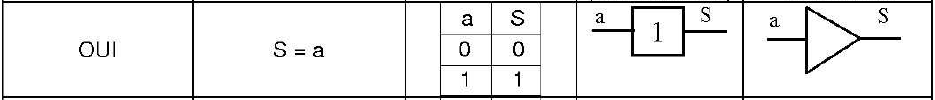
\includegraphics[width=.9\textwidth]{png/oui_logi}

\textit{Fonction OUI -- Table de vérité et logigramme}
\end{center}
\end{minipage} \hfill
\begin{minipage}[c]{.3\linewidth}
\begin{center}
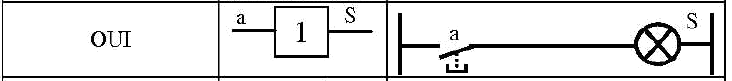
\includegraphics[width=.9\textwidth]{png/oui_elec}

\textit{Fonction OUI en technologie électrique}
\end{center}
\end{minipage} \hfill
\begin{minipage}[c]{.3\linewidth}
\begin{center}
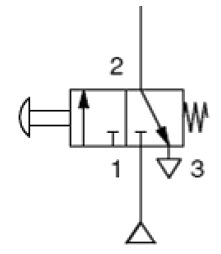
\includegraphics[width=.9\textwidth]{png/oui_pneu}

\textit{Fonction OUI en technologie pneumatique}
\end{center}
\end{minipage}
\end{exemple}


\subsubsection{Fonction NON -- appelée complément}
\begin{defi}
\textbf{Fonction NON -- appelée complément}

\begin{minipage}[c]{.45\linewidth}
\begin{eqnarray*}
B &\longmapsto& B\\
a &\longmapsto& \overline{a}
\end{eqnarray*}
Il faut lire $\overline{a}$ : NON a.
\end{minipage} \hfill
\begin{minipage}[c]{.45\linewidth}
\begin{center}
\begin{tabular}{|c||c|}
\hline
$a$ & $\overline{a}$ \\
\hline
0 & 1 \\
\hline
1 & 0 \\
\hline
\end{tabular}
\end{center}
\end{minipage}
\end{defi}

\begin{exemple}
Fonction NON.

\begin{minipage}[c]{.3\linewidth}
\begin{center}
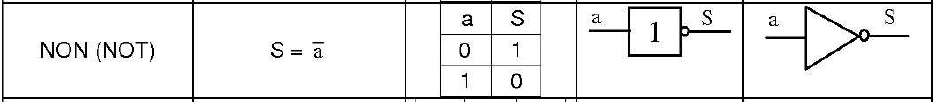
\includegraphics[width=.9\textwidth]{png/non_logi}

\textit{Fonction NON -- Table de vérité et logigramme}
\end{center}
\end{minipage} \hfill
\begin{minipage}[c]{.3\linewidth}
\begin{center}
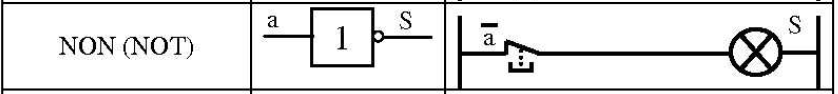
\includegraphics[width=.9\textwidth]{png/non_elec}

\textit{Fonction NON en technologie électrique}
\end{center}
\end{minipage} \hfill
\begin{minipage}[c]{.3\linewidth}
\begin{center}
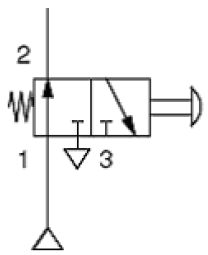
\includegraphics[width=.9\textwidth]{png/non_pneu}

\textit{Fonction NON en technologie pneumatique}
\end{center}
\end{minipage}
\end{exemple}


\subsubsection{Fonction ET -- Produit booléen}

\begin{defi}
\textbf{Fonction ET -- Produit booléen}

\begin{minipage}[c]{.45\linewidth}
\begin{eqnarray*}
B \times B &\longmapsto& B\\
(a,b) &\longmapsto& a \cdot b
\end{eqnarray*}
Il faut lire $a$ ET $b$. 
\end{minipage} \hfill
\begin{minipage}[c]{.45\linewidth}
\begin{center}
\begin{tabular}{|c|c||c|}
\hline
$a$ & $b$ & $a\cdot b$ \\
\hline
0 & 0 & 0 \\ \hline
0 & 1 & 0 \\ \hline
1 & 0 & 0 \\ \hline
1 & 1 & 1 \\ \hline
\end{tabular}
\end{center}
\end{minipage}
\end{defi}

\begin{exemple}
Fonction ET.

\begin{minipage}[c]{.3\linewidth}
\begin{center}
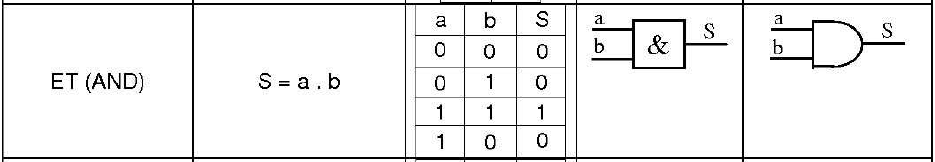
\includegraphics[width=.9\textwidth]{png/et_logi}

\textit{Fonction ET -- Table de vérité et logigramme}
\end{center}
\end{minipage} \hfill
\begin{minipage}[c]{.3\linewidth}
\begin{center}
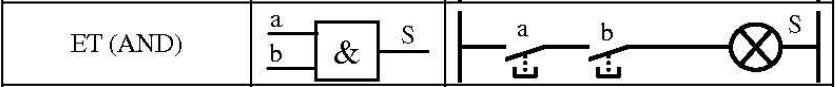
\includegraphics[width=.9\textwidth]{png/et_elec}

\textit{Fonction ET en technologie électrique}
\end{center}
\end{minipage} \hfill
\begin{minipage}[c]{.3\linewidth}
\begin{center}
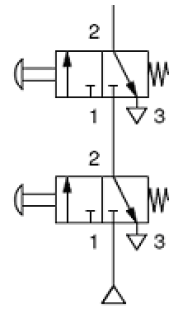
\includegraphics[width=.9\textwidth]{png/et_pneu}

\textit{Fonction ET en technologie pneumatique}
\end{center}
\end{minipage}
\end{exemple}


\subsubsection{Fonction OU -- Somme booléenne}


\begin{defi}
\textbf{Fonction OU -- Somme booléenne}

\begin{minipage}[c]{.45\linewidth}
\begin{eqnarray*}
B \times B &\longmapsto& B\\
(a,b) &\longmapsto& a + b
\end{eqnarray*}
Il faut lire $a$ OU $b$. 
\end{minipage} \hfill
\begin{minipage}[c]{.45\linewidth}
\begin{center}
\begin{tabular}{|c|c||c|}
\hline
$a$ & $b$ & $a+ b$ \\
\hline
0 & 0 & 0 \\ \hline
0 & 1 & 1 \\ \hline
1 & 0 & 1 \\ \hline
1 & 1 & 1 \\ \hline
\end{tabular}
\end{center}
\end{minipage}
\end{defi}

\begin{exemple}
Fonction OU.

\begin{minipage}[c]{.3\linewidth}
\begin{center}
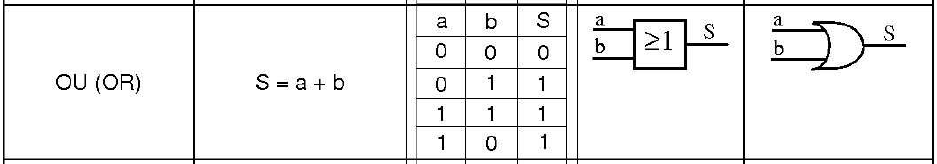
\includegraphics[width=.9\textwidth]{png/ou_logi}

\textit{Fonction OU -- Table de vérité et logigramme}
\end{center}
\end{minipage} \hfill
\begin{minipage}[c]{.3\linewidth}
\begin{center}
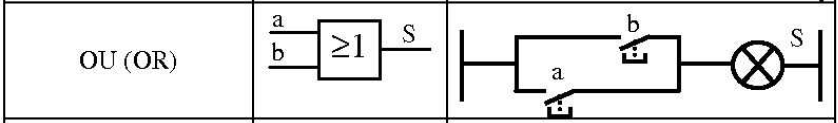
\includegraphics[width=.9\textwidth]{png/ou_elec}

\textit{Fonction OU en technologie électrique}
\end{center}
\end{minipage} \hfill
\begin{minipage}[c]{.3\linewidth}
\begin{center}
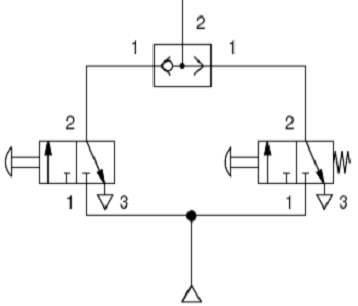
\includegraphics[width=.9\textwidth]{png/ou_pneu}

\textit{Fonction OU en technologie pneumatique}
\end{center}
\end{minipage}
\end{exemple}

\subsubsection{Propriétés des opérateurs de base de l'algèbre de Boole}

\begin{prop}
\textbf{Commutativité}

\begin{minipage}[c]{.45\linewidth}
$$ a+b = b+a$$
\end{minipage}\hfill
\begin{minipage}[c]{.45\linewidth}
$$ a\cdot b = b\cdot a$$
\end{minipage}
\end{prop}


\begin{prop}
\textbf{Distributivité}

\begin{minipage}[c]{.45\linewidth}
$$ a\cdot (b+c) = a\cdot b+a \cdot c$$
\end{minipage}\hfill
\begin{minipage}[c]{.45\linewidth}
$$ a+(b\cdot c) = (a+b) \cdot (a+c)$$
\end{minipage}
\end{prop}

\begin{prop}
\textbf{Associativité}

\begin{minipage}[c]{.45\linewidth}
$$ a + (b+c) = (a+b)+c = a+b+c$$
\end{minipage}\hfill
\begin{minipage}[c]{.45\linewidth}
$$ a \cdot (b\cdot c) = (a\cdot b)\cdot c = a \cdot b\cdot c$$
\end{minipage}
\end{prop}

\begin{prop}
\textbf{Élément neutre}

\begin{minipage}[c]{.45\linewidth}
$$ a + 0 = a$$
\end{minipage}\hfill
\begin{minipage}[c]{.45\linewidth}
$$ a\cdot 1 = a$$
\end{minipage}
\end{prop}

\begin{prop}
\textbf{Élément absorbant}

\begin{minipage}[c]{.45\linewidth}
$$ a + 1 = 1$$
\end{minipage}\hfill
\begin{minipage}[c]{.45\linewidth}
$$ a\cdot 0 = 0$$
\end{minipage}
\end{prop}



\begin{prop}
\textbf{Complémentarité}

\begin{minipage}[c]{.45\linewidth}
$$ a + \overline{a} = 1$$
\end{minipage}\hfill
\begin{minipage}[c]{.45\linewidth}
$$ a\cdot \overline{a} = 0$$
\end{minipage}

Par ailleurs $\overline{\overline{a}}=a$.
\end{prop}



\begin{prop}
\textbf{Idem potence}

\begin{minipage}[c]{.45\linewidth}
$$ a + a = a$$
\end{minipage}\hfill
\begin{minipage}[c]{.45\linewidth}
$$ a\cdot a = a$$
\end{minipage}
\end{prop}


\begin{prop}
\textbf{Identités remarquables}

Absorption : 
$$ a + a\cdot b = a$$

Inclusion :
$$
a+\overline{a}\cdot b = a+b
$$
\end{prop}

\subsubsection{Théorème de Morgan}
\begin{theo}
$$
\overline{\sum\limits_{i=1}^{n} a_i} = \prod\limits_{i=1}^n \overline{a_i}
$$

$$
\overline{\prod\limits_{i=1}^{n} a_i} = \sum\limits_{i=1}^n \overline{a_i}
$$
\end{theo}

\begin{exemple}
Déterminer les expressions complémentaires $\overline{P}$ et $\overline{Q}$ des expressions suivantes : 
$P = x\cdot y \cdot (z + \overline{t})$ et $Q=\overline{x}\cdot\overline{y} + y + x\cdot t$.
\end{exemple}

\section{Fonctions logiques}

Un système combinatoire est décrit par une fonction logique qui permet de définir de manière unique la sortie pour une combinaison des entrées. 

\subsection{Table de vérité}
La table de vérité d'une fonction logique est une écriture systématique qui consiste à décrire toutes les combinaison des variables et à y associer les valeurs correspondantes de la fonction. 

\begin{exemple}
La table de vérité pour les lampes $L_1$, $L_2$, $L_3$, $L_4$ de l'éclairage d'escalier est la suivante :
\begin{center}
\begin{tabular}[c]{|c|c|c||c|c|c|c|}
\hline 
$a$ & $b$ & $c$ & $L_1$ & $L_2$ & $L_3$ & $L_4$ \\
\hline \hline
0 & 0 & 0 & 0 & 0 & 0 & 0 \\ \hline
0 & 0 & 1 & 0 & 0 & 0 & 1 \\ \hline
0 & 1 & 1 & 0 & 0 & 1 & 1 \\ \hline
0 & 1 & 0 & 0 & 1 & 1 & 0 \\ \hline
1 & 1 & 0 & 1 & 1 & 0 & 0 \\ \hline
1 & 1 & 1 & 1 & 1 & 1 & 1 \\ \hline
1 & 0 & 1 & 1 & 0 & 0 & 1 \\ \hline
1 & 0 & 0 & 1 & 0 & 0 & 0 \\ \hline 
\end{tabular}
\end{center}

Compléter la table de vérité suivante et vérifier les théorèmes de De Morgan pour deux variables.
\begin{center}
\begin{tabular}[c]{|c|c||c|c|c|c|}
\hline
$a$ & $b$ & $\overline{a\cdot b}$ & $\overline{a} + \overline{b}$ & $\overline{a+b}$ & $\overline{a}\cdot\overline{b}$ \\
\hline \hline 
0 & 0 & & & & \\ \hline
0 & 1 & & & & \\ \hline
1 & 1 & & & & \\ \hline
1 & 1 & & & & \\ \hline
\end{tabular}
\end{center}

\end{exemple}

Il est possible à l'aide de la table de vérité de définir une équation donnant les variables de sortie en fonction des variables d'entrée. Il existe 2 modes d'écriture particuliers : 
\begin{itemize}
\item somme canonique (somme de produit) : $S=a\cdot b + c\cdot d$;
\item produit canonique (produit de sommes) : $S=(a+b) \cdot (c+d)$.
\end{itemize}

\begin{methode}
\textbf{Détermination de la somme canonique}

Pour chaque ligne où la sortie vaut 1, déterminer la combinaison d'entrées correspondante à l'aide de l'opérateur ET puis sommer ces combinaisons. 
\end{methode}


\begin{exemple}
Donner l'expression sous forme canonique de $L_1$ et $L_2$ à partir de la table de vérité précédente. 
\end{exemple}

\begin{rem}
On utilise la forme de sommes canoniques si le nombre de 1 est inférieur au nombre de 0. Il est souvent nécessaire de simplifier ces équations pour réaliser technologiquement ces fonctions (voir plus loin).
\end{rem}

\begin{methode}
\textbf{Détermination du produit canonique}

Déterminer l'expression de $\overline{S}$ ce qui revient à :
Déterminer la combinaison d'entrées pour chaque ligne où la sortie vaut 0, les sommer, puis passez au complémentaire en utilisant les théorèmes de De Morgan. 
\end{methode}

\begin{exemple}
Donner l'expression sous forme de produit canonique de $L_1$ et $L_2$.
\end{exemple}

\begin{rem}
Cette méthode est utile lorsque la sortie comporte peu de 0 et beaucoup de 1 ou lorsque l'on recherche la fonction complémentaire. 
\end{rem}

\section{Réorganisation (Simplification) des fonctions logiques}
La simplification des expressions logiques est destinée à économiser le matériel nécessaire à la réalisation (utilisation d'un composant réalisant plusieurs fonctions identiques) ou diminuer l'importance des équations programmées.

\subsection{Cellules universelles}
\begin{defi}

Une cellule (ou fonction) est dite "universelle" si elle permet de réaliser les fonctions ET, OU, NON. Il est alors possible de réaliser toutes les fonctions logiques à l'aide de cette seule cellule. 
\end{defi}

\begin{exemple}
Les cellules NAND (non et -- $a NAND b = \overline{a\cdot b}$) et NOR (non ou -- $a NOR b = \overline{a + b}$) sont des cellules universelles. 

Réalisation de la fonction NON : $ NON(a) = \overline{a} = \overline{a\cdot a}$. Besoin d'une seule cellule NAND. 
 
Réalisation de la fonction ET : $ a ET b = a\cdot b= \overline{\overline{a\cdot b}} $. Besoin de deux cellules NAND en cascade. 

Réalisation de la fonction OU : $ a OU b = a+ b= \overline{\overline{a+b}}= \overline{\overline{a}\cdot\overline{b}} $. Besoin de trois cellules NAND en cascade. 

De même, la cellule NOR est universelle.
\end{exemple}

\begin{exemple}
Écrire l'expression logique suivante uniquement avec des opérateurs NAND puis indiquer le nombre minimal d'opérateurs utilisés.
$$
F=c\cdot (\overline{a}+\overline{b})
$$
\end{exemple}

\subsection{Simplification algébrique d'une fonction}
Il s'agit d'utiliser les propriétés, théorèmes et identités remarquables de l'algèbre de Boole afin de simplifier une équation. Cette méthode n'est pas forcément simple à utiliser et demande beaucoup d'intuition.

\begin{exemple}
$$F(a,b,c) = \overline{a}\cdot \overline{b} \cdot c + a \cdot \overline{b} \cdot c + \overline{a}\cdot b \cdot c = \overline{a}\cdot c \cdot (\overline{b}+b) + a\cdot \overline{b}\cdot c = \overline{a}\cdot c + a\cdot \overline{b}\cdot c = c(\overline{a}+a\cdot \overline{b}) = c\left(\overline{a}(1+\overline{b}) + a \cdot \overline{b}\right) = c\cdot (\overline{a}+\overline{b})$$
\end{exemple}

\begin{exemple}
Simplifier par cette méthode l'expression des lampes $L_1$ et $L_2$. 
\end{exemple}

\subsection{Simplification graphique : Tableaux de Karnaugh}
Le tableau de Karnaugh est une présentation particulière de la table de vérité permettant de simplifier graphiquement une expression analytique. 

\subsubsection{Construction du tableau de Karnaugh}
Un tableau de Karnaugh comporte autant d'entrées qu'il y a de variables et associe une case à chaque combinaison de ces variables. Pour une fonction de $n$ variables, un tableau de Karnaugh comporte donc $2^n$ cases. Le tableau répartit les entrées en ligne et en colonne de manière à n'obtenir qu'un seul changement d'une entrée au passage d'un case à une case mitoyenne (code binaire réfléchi obtenu par symétries). Ainsi pour une fonction à $n$ variables, le passage d'une case adjacente à une autre correspond au changement de valeur d'une seule variable. 

%\begin{center}
%\begin{tabular}{|c|c|}
%\multicolumn{2}{c}{a} \\
%\multicolumn{1}{c}{0} & \multicolumn{1}{c}{1} \\
%\hline
%F(0) & F(1) \\
%\hline
%\end{tabular}
%
%\textit{Tableau à 1 variable}
%\end{center}
%
%
%\begin{center}
%\begin{tabular}{|c|c|c|c|}
%\multicolumn{2}{c}{}&\multicolumn{2}{c}{a} \\
%\multicolumn{2}{c}{}&\multicolumn{1}{c}{0}&\multicolumn{1}{c}{1} \\
%\hline
%
%\hline
%\end{tabular}
%
%\textit{Tableau à 2 variables}
%\end{center}

\begin{center}
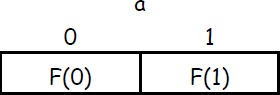
\includegraphics[width=.3\textwidth]{png/fig_10}

\textit{Tableau à 1 variable}

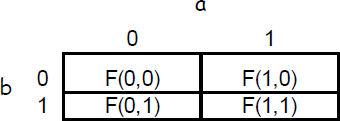
\includegraphics[width=.35\textwidth]{png/fig_11}

\textit{Tableau à 2 variables}

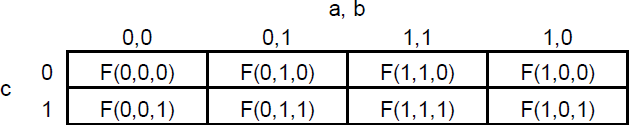
\includegraphics[width=.6\textwidth]{png/fig_12}

\textit{Tableau à 3 variables}

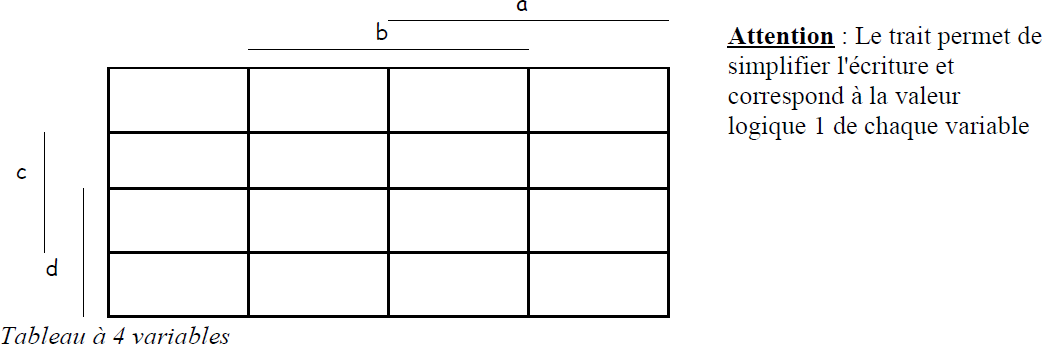
\includegraphics[width=.6\textwidth]{png/fig_13}

\textit{Tableau à 4 variables}
\end{center}

\begin{exemple}
Écrire le tableau de Karnaugh des lampes $L_1$ et $L_2$. 
\end{exemple}


\subsubsection{Simplification par tableau de Karnaugh}
Les simplifications d'une fonction à l'aide de son tableau de Karnaugh consistent à faire des regroupements de 1 adjacent par puissance de deux. Ces regroupements doivent être les plus gros possibles et en nombre minimum afin d'obtenir l'expression la plus simple possible. Des recoupements entre les regroupements sont possibles. 

Pour que la simplification ait lieu, les regroupements doivent être disposés de manière symétrique par rapport aux axes de symétrie du tableau. Ces axes correspondent aux symétries effectuées pour établir le code Gray. 

\subsubsection{Exemple détaillé}
Considérons la fonction $F(a,b,c) = \overline{a}\cdot \overline{b}\cdot c + a \cdot \overline{b} \cdot c + \overline{a} \cdot b \cdot c$ étudiée précédemment, décrite par sa table de vérité et établissons son tableau de Karnaugh. 

Un premier regroupement de 1 apparaît facilement. Dans ce regroupement, la variable $b$ intervient sous forme de 1 et de 0 et peut être ignorée. 

\begin{center}
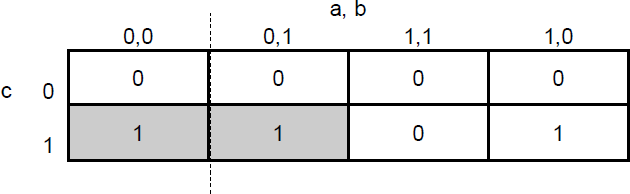
\includegraphics[width=.6\textwidth]{png/fig_14}
\end{center}

Ce regroupement est équivalent à $\overline{a}\cdot c$. 

En effet, nous avons pour ces deux cases : $(\overline{a}\cdot\overline{b}\cdot c)+(\overline{a}\cdot b \cdot c)= \overline{a}\cdot c (\overline{b}+b)=\overline{a}\cdot c$.

Le résultat fait normalement intervenir deux variables parce qu'il y a trois variables d'entrée et que la simplification s'est effectuée au moyen d'un regroupement de $2^1$ cases. 

Un deuxième regroupement peut être effectué si on prend en compte la symétrie verticale (ceci correspond dans le cadre des tableaux à 3 ou 4 variables à considérer les colonnes ou les lignes extrêmes adjacentes).

\begin{center}
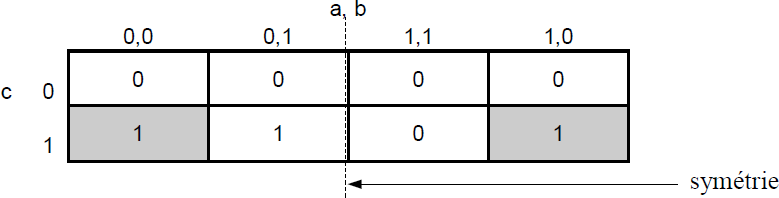
\includegraphics[width=.6\textwidth]{png/fig_15}
\end{center}

Ce regroupement est équivalent à $\overline{b}\cdot c $.

En effet, nous avons pour ces deux cases : $(\overline{a}\cdot \overline{b}\cdot c)+(a\cdot \overline{b}\cdot c)=\overline{b}\cdot c(\overline{a}\cdot a) = \overline{b}\cdot c$. Le résultat fait normalement intervenir deux variables parce qu'il y a trois variables d'entrée et que la simplification s'est effectuée au moyen d'un groupement de $2^1$ cases. La fonction $F(a,b,c)$ s'écrit donc : $F(a,b,c)=\overline{a}\cdot c + \overline{b}\cdot c =(\overline{a} + \overline{b}) \cdot c$.

\begin{rem}
Il est possible de faire des regroupements de 0 pour obtenir la fonction complémentée. 
\end{rem}

\begin{exemple}
Simplifier l'expression des lampes $L_1$ et $L_2$ à partir des tableaux de Karnaugh.
\end{exemple}

\subsubsection{Cas des fonctions incomplètes}
Le cas des fonctions incomplètes (ou incomplètement spécifiées) peut apparaître comme un cas particulier. En réalité, on peut considérer qu'en pratique c'est le cas le plus fréquent. En effet : 
\begin{itemize}
\item soit la valeur de la fonction n'a pas réellement d'importance pour le problème considéré;
\item soit certains combinaisons de variables sont physiquement impossibles.
\end{itemize}
Dans ces conditions, la case correspondant à la combinaison non spécifiée sera marquée par un symbole $\Phi$ ou laissée vide. 

La démarche de simplification d'une telle fonction se déroule de la même manière que précédemment. Il faut choisir des regroupements de $2^1$, $2^2$, ... cases. Si le regroupement se fait par les 1 (respectivement 0) alors les cases contenant $\Phi$ qui interviennent dans le regroupement prenant la valeur 1 (respectivement 0), et les cases ne contenant pas $\Phi$ qui interviennent dans le regroupement prennent la valeur 0 (respectivement 1). La fonction est ainsi complètement spécifiée.

\begin{rem}
Il n'est pas nécessaire de faire intervenir tous les $\Phi$ dans les regroupements. 
\end{rem}

\begin{exemple}
Simplifier le tableau suivant. 

\begin{center}
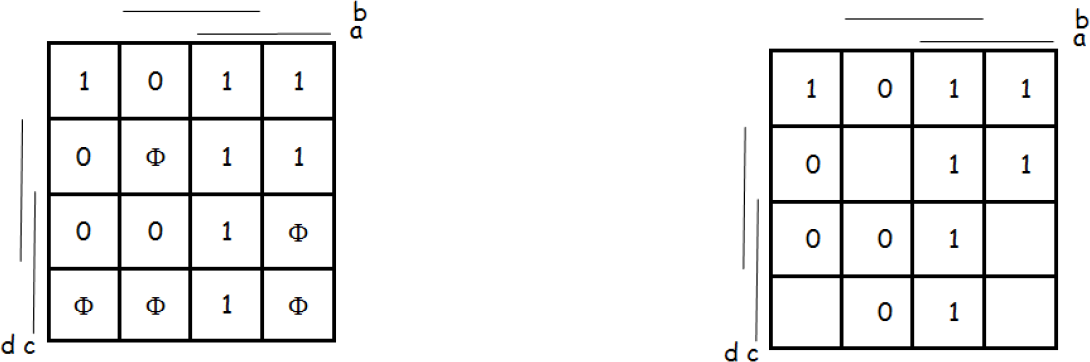
\includegraphics[width=.6\textwidth]{png/fig_16}
\end{center}

\end{exemple}

\section{Représentation des fonctions logiques}
Dans un système combinatoire : 
\begin{itemize}
\item les variables d'entrée sont des informations qui décrivent à un moment donnée l'état de certaines parties (position d'un chariot, d'un outil, ...)
\item les variables de sortie permettent de décrire l'état dans lequel doivent se retrouver les organes récepteurs. 
\end{itemize}

Une fois l'expression logique obtenue et simplifiée, il est possible d'exprimer graphiquement le comportement du système combinatoire. On utilise pour cela en général le logigramme ou le schéma électrique. On peut également utiliser un schéma pneumatique ou électronique.

\subsection{Logigramme}

%Un logigramme est une représentation logique 


\begin{center}
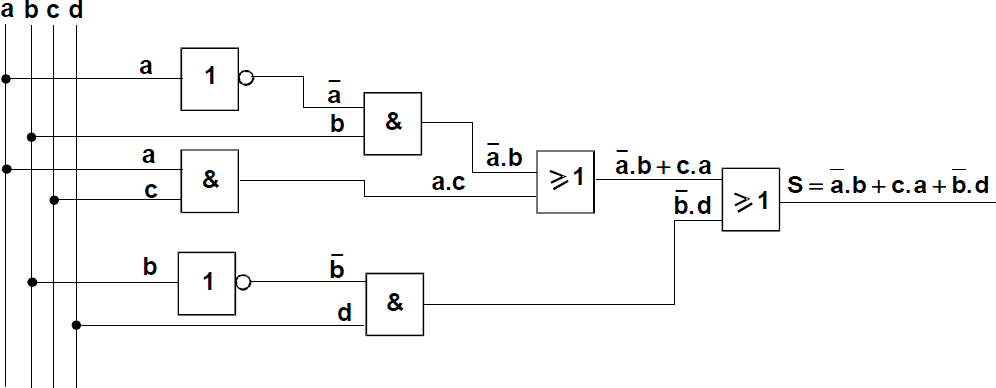
\includegraphics[width=.6\textwidth]{png/fig_17}
\end{center}

\begin{center}
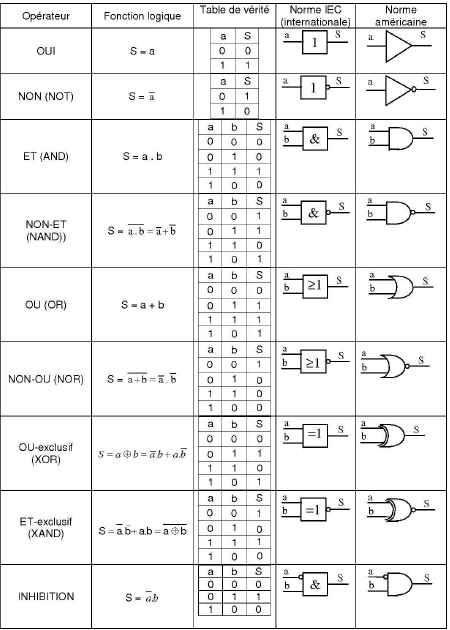
\includegraphics[height=\textheight]{png/fig_18}
\end{center}




\begin{thebibliography}{2}
\bibitem{dv}{Supports de cours de David Violeau, Lycée Saint-Louis, Paris}
\bibitem{fm}{Supports de cours de Florestan Mathurin, Lycée Bellevue, Toulouse}
%\bibitem{jpp}{Supports de cours de Jean-Pierre Pupier, Lycée Rouvière, Toulon}

\end{thebibliography}

\end{document}